\documentclass[11pt]{amsbook}
\usepackage[turkish]{babel}

\usepackage{../Ceyhun}	% ------------------------
\usepackage{../amsTurkish}


\usepackage{lipsum}



\begin{document}

    \hPage{098}
    \begin{figure}[htb]
	    \centering
	    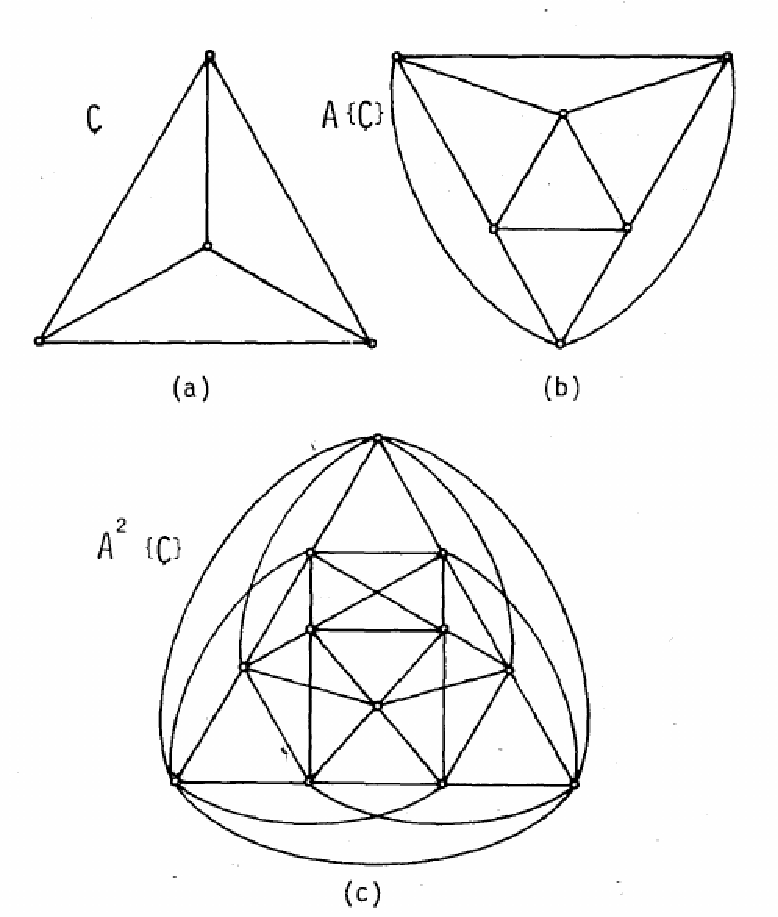
\includegraphics[width=0.65\textwidth]{images/ceyhun098-fig01}
	    \caption{ $a)$Ç\ , b) $A$ \{ Ç \}, $c) \  A^2$\{ Ç \}}
    \end{figure}
    \begin{proof}
        Tanımdan, ayrıt çizgesinde $a$ sayıda düğüm bulunduğu bilinmektedir. $d_i$ düğümüne çakışık olan $k_i$ sayıdaki ayrıt, $A$ \{Ç$(d,a)\}$ ayrıtların
    \end{proof}
\end{document}